\documentclass[conference]{IEEEtran}

% Biên dịch bằng XeLaTeX hoặc LuaLaTeX để hỗ trợ tiếng Việt qua fontspec.
\usepackage{fontspec}
\setmainfont{DejaVu Serif}
\setsansfont{DejaVu Sans}
\usepackage{graphicx}
\usepackage{longtable}
\usepackage{float}
\usepackage{placeins}
\usepackage{amsmath}
\usepackage{hyperref}
\usepackage[numbers,sort&compress]{natbib}

% Việt hoá nhãn abstract và index terms trong IEEEtran
\renewcommand{\abstractname}{Tóm tắt}
\renewcommand{\IEEEkeywordsname}{Từ khóa}

\title{Kiểm chứng tính toàn vẹn dữ liệu trong Data Pipeline nhiều giai đoạn\\
bằng Hash-linked Tamper-evident Ledger: một đánh giá bán thực nghiệm}

\author{
\IEEEauthorblockN{Nguyễn Ngọc Sơn}
\IEEEauthorblockA{Học viện Kỹ thuật Mật mã\\
Email: [CHAT4P016@actvn.edu.vn]}
}
\begin{document}

\maketitle

\begin{abstract}
Bài báo trình bày một đánh giá bán thực nghiệm đối với cơ chế Hash-linked
Tamper-evident Ledger nhằm kiểm chứng tính toàn vẹn dữ liệu trong Data
Pipeline nhiều giai đoạn. Cơ chế này ghi nhận bằng chứng toàn vẹn ở từng
giai đoạn, liên kết các block ledger bằng \texttt{previous\_hash}, và sử
dụng bộ kiểm chứng để phát hiện sửa đổi sau xử lý. Kết quả thực nghiệm hỗ
trợ các giả thuyết chính trong phạm vi giới hạn, đồng thời được diễn giải
cùng các mối đe dọa đến tính hợp lệ.
\end{abstract}

\begin{IEEEkeywords}
Tính toàn vẹn dữ liệu, tamper-evident ledger, hash chain, Data Pipeline,
đánh giá bán thực nghiệm, an toàn thông tin, Data Lineage.
\end{IEEEkeywords}

\section{Giới thiệu}\label{sec:gioithieu}

Data Pipeline đã trở thành thành phần quan trọng trong các hệ thống
thông tin phục vụ vận hành và phân tích dữ liệu. Một pipeline điển hình
tiếp nhận dữ liệu nguồn, xử lý qua các tầng trung gian, lưu trữ kết quả
đã chuẩn hóa và cung cấp dữ liệu cho báo cáo hoặc ứng dụng hạ nguồn.
Trong nhiều kiến trúc lakehouse hoặc warehouse, vòng đời này thường được
biểu diễn qua các giai đoạn như Source--Bronze--Silver--Gold~\citep{databricksMedallion}. Tuy các giai đoạn
này giúp tổ chức dữ liệu rõ ràng hơn, chúng không tự động bảo đảm rằng
dữ liệu sẽ không bị thay đổi sau khi pipeline đã hoàn tất. Các nền tảng
dữ liệu hiện đại như Delta Lake hỗ trợ nhật ký giao dịch và quản lý dữ
liệu theo phiên bản, nhưng bài toán kiểm chứng độc lập sau xử lý vẫn cần
một lớp bằng chứng integrity rõ ràng hơn trong ngữ cảnh an toàn thông
tin \citep{databricksDelta,iso27001}.

Đây là vấn đề thuộc phạm vi an toàn thông tin và bảo đảm thông tin. Nếu
người dùng có quyền cao, tài khoản bị xâm nhập hoặc người có quyền truy cập nội bộ chỉnh sửa dữ
liệu sau khi pipeline chạy xong, công cụ điều phối vẫn có thể hiển
thị trạng thái thành công. Cơ chế giám sát thông thường có thể xác nhận
rằng tác vụ đã chạy, nhưng không nhất thiết kiểm chứng độc lập rằng dữ liệu
lưu trữ sau đó vẫn còn nguyên vẹn. Nhật ký kiểm toán cơ sở dữ liệu có thể hỗ trợ điều
tra, nhưng thường nằm trong cùng ranh giới quản trị với dữ liệu được bảo
vệ. Mã kiểm tra ở tầng ứng dụng có thể phát hiện sai lệch đơn giản, nhưng
nếu không được liên kết theo chuỗi giữa các giai đoạn thì khó cung cấp bằng
chứng truy vết rõ ràng đến transformation bị ảnh hưởng.

Nghiên cứu này là một hướng tiếp cận nhẹ hơn: Hash-linked
Tamper-evident Ledger. Cơ chế tamper-evident không ngăn chặn trực tiếp
việc chỉnh sửa dữ liệu. Thay vào đó, nó tạo ra bằng chứng để phát hiện
rằng việc chỉnh sửa đã xảy ra. Hash-linked Ledger lưu các bản ghi bằng
chứng theo thứ tự, trong đó mỗi block chứa hash của block trước đó~\citep{merkle1978}. Nếu
nội dung của block hoặc liên kết previous\_hash bị thay đổi, quá trình
verification về sau có thể phát hiện chuỗi không còn khớp. Cách liên kết
bằng hash kế thừa ý tưởng cốt lõi của blockchain
\citep{nakamoto2008bitcoin}, nhưng nghiên cứu này chỉ đánh giá một ledger
nhẹ, không bao gồm consensus, smart contract hoặc mạng phi tập trung đầy
đủ.

\subsection{Khoảng trống nghiên
cứu}\label{sec:khoangtrong}

Một số cơ chế hiện có đã giải quyết từng phần của bài toán toàn vẹn dữ
liệu. Nhật ký kiểm toán cơ sở dữ liệu ghi lại thao tác, nhưng quản trị viên có quyền
cao có thể tác động đến cả dữ liệu và log~\citep{schneierKelsey1998}. Mã kiểm tra ở tầng ứng dụng có
thể xác thực một ảnh chụp trạng thái dữ liệu, nhưng thường bị cô lập và không bảo
toàn quan hệ giữa các giai đoạn. Blockchain phi tập trung đầy đủ có thể cung
cấp đặc tính bất biến mạnh hơn thông qua consensus và nhiều nút sao
chép, nhưng chi phí phát sinh vận hành và độ phức tạp kiến trúc thường vượt quá
nhu cầu của một bài toán kiểm chứng integrity nội bộ trong Data
Pipeline. Pipeline monitoring quan sát trạng thái thực thi, nhưng không
nhất thiết cung cấp bằng chứng kiểm chứng sau khi pipeline đã hoàn tất.

Khoảng trống mà bài báo này tập trung là thiếu một đánh giá có kiểm soát
về cơ chế Hash-linked Ledger nhẹ cho kiểm chứng tính toàn vẹn của Data
Pipeline nhiều giai đoạn. Nghiên cứu xem xét liệu cơ chế này có phát hiện
được các kịch bản tampers được định nghĩa trước hay không, có xác định
được block sai lệch đầu tiên và ngữ cảnh lineage liên quan hay không, và
chi phí phát sinh bổ sung thay đổi như thế nào trong một môi trường thực nghiệm
bị ràng buộc.

\subsection{Câu hỏi nghiên
cứu}\label{sec:cauhoi}

Nghiên cứu được dẫn dắt bởi bốn câu hỏi nghiên cứu:

\begin{itemize}
\item
  \textbf{RQ1:} Cơ chế Hash-linked Ledger và bộ kiểm chứng có phát hiện
  được các sửa đổi trái phép đối với dữ liệu pipeline, nội dung ledger và
  liên kết chuỗi hay không?
\item
  \textbf{RQ2:} Cơ chế này có xác định được block sai lệch đầu tiên, giai đoạn bị
  ảnh hưởng và lineage event liên quan hay không?
\item
  \textbf{RQ3:} Cơ chế này tạo thêm chi phí phát sinh thời gian xử lý như thế nào
  khi số lượng bản ghi thay đổi?
\item
  \textbf{RQ4:} Những biến không kiểm soát được trong môi trường thực
  nghiệm giới hạn sức mạnh kết luận ra sao?
\end{itemize}

\subsection{Đóng góp}\label{sec:donggop}

Bài báo có ba đóng góp chính. Thứ nhất, nghiên cứu định nghĩa một cơ chế
tamper-evident có phạm vi rõ ràng cho kiểm chứng integrity của Data
Pipeline bằng batch\_hash, block\_hash, liên kết \texttt{previous\_hash} và lineage
event ở từng giai đoạn. Thứ hai, nghiên cứu thiết kế một đánh giá bán thực
nghiệm với điều kiện sạch, điều kiện bị tamper và điều kiện benchmark.
Thứ ba, nghiên cứu báo cáo quan sát thực nghiệm cùng các giới hạn
validity, thay vì tuyên bố quá mức rằng cơ chế này đạt tính bất biến như
Blockchain đầy đủ hoặc đưa ra kết luận nhân quả mạnh.

\section{Phương pháp nghiên
cứu}\label{sec:phuongphap}

\subsection{Biện minh lựa chọn thiết kế bán thực
nghiệm}\label{sec:bienminh}

Nghiên cứu này sử dụng phương pháp bán thực nghiệm (quasi-experimental)~\citep{shadishCook2002}
vì can thiệp kỹ thuật có thể được triển khai và đo lường, nhưng môi
trường thực nghiệm không thể được kiểm soát hoàn toàn. Một thực nghiệm
đúng nghĩa (true experiment) đòi hỏi phân bổ ngẫu nhiên, tài nguyên tính toán cố định, điều
kiện mạng ổn định, các lần chạy lặp lại trong trạng thái tài nguyên
giống hệt nhau và tập đối tượng tấn công đại diện cho thực tế. Những giả
định này không khả thi trong môi trường Databricks được sử dụng trong
nghiên cứu.

Thực nghiệm kiểm soát các yếu tố có thể kiểm soát được: cấu trúc
pipeline, seed sinh dữ liệu tổng hợp, danh sách kịch bản tamper, logic kiểm chứng, tập biến đo lường và thứ tự quy trình. Đồng thời, nghiên
cứu ghi nhận các yếu tố không thể kiểm soát: lập lịch trên nền tảng đám mây, trạng
thái khởi động, cache, độ trễ mạng và việc các kịch bản tamper là đại diện gần đúng (proxy)
do nhà nghiên cứu thiết kế, không phải mẫu ngẫu nhiên của không gian tấn công thực
tế. Vì vậy, kết quả được diễn giải là bằng chứng bán thực nghiệm về quan
hệ giữa điều kiện can thiệp và kết quả quan sát được, không phải kết luận nhân quả
phổ quát.

\subsection{Điều kiện can thiệp và điều kiện đối chứng}\label{sec:extra1}

Điều kiện can thiệp (treatment) là việc bổ sung Hash-linked Tamper-evident Ledger, lineage
recorder và bộ kiểm chứng vào một Data Pipeline chuẩn. Điều kiện đối chứng phụ thuộc vào câu hỏi nghiên cứu. Đối với phát hiện và truy vết, trạng thái pipeline sạch, không có kịch bản tamper, đóng
vai trò điều kiện đối chứng trước can thiệp. Đối với chi phí phát sinh, pipeline baseline không có
ledger và thành phần đo lường và kiểm chứng đóng vai trò điều kiện đối chứng
không tương đương.

\begin{figure}[t]
\centering
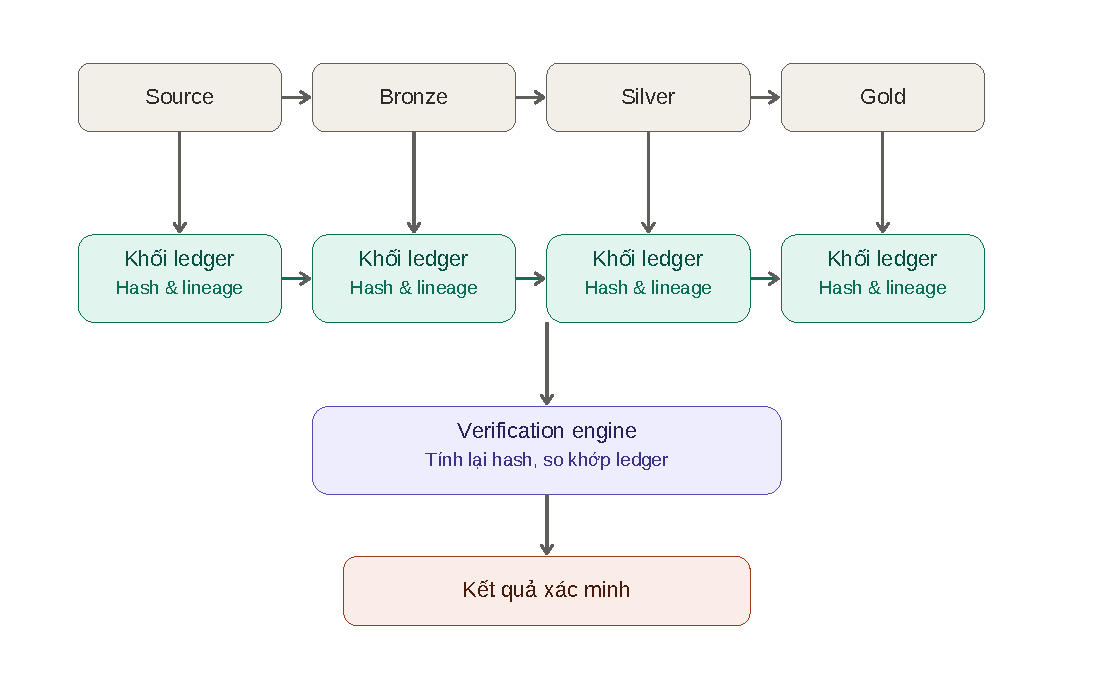
\includegraphics[width=\columnwidth]{images/kien_truc_ledger.pdf}
\caption{Hash-linked Tamper-evident Ledger cho Data Pipeline nhiều giai đoạn.}
\label{fig:architecture}
\end{figure}

\subsection{Giả thuyết nghiên cứu}\label{sec:giathuyet}

Tương ứng với bốn câu hỏi nghiên cứu, bốn giả thuyết được phát biểu
trong Bảng~\ref{tab:hypotheses}.

\begin{table}[!t]
\centering
\caption{Giả thuyết nghiên cứu}
\label{tab:hypotheses}
\begin{tabular}{|l|p{\dimexpr\columnwidth-1.2cm-6\tabcolsep\relax}|}
\hline
\textbf{Mã} & \textbf{Giả thuyết} \\
\hline
H1 & Treatment phát hiện tất cả kịch bản tamper được định nghĩa trước,
trong khi điều kiện sạch vẫn hợp lệ. \\
\hline
H2 & Treatment xác định được block sai lệch đầu tiên và liên kết được với
lineage event tương ứng. \\
\hline
H3 & Treatment làm tăng thời gian xử lý so với pipeline baseline, và
chi phí phát sinh thay đổi theo số lượng bản ghi. \\
\hline
H4 & Các biến không kiểm soát được khiến nghiên cứu không thể đưa ra kết
luận nhân quả mạnh như thực nghiệm đúng nghĩa (true experiment). \\
\hline
\end{tabular}
\end{table}
\subsection{Biến nghiên cứu}\label{sec:bienso}

Các biến độc lập gồm kịch bản tamper, số lượng bản ghi, giai đoạn pipeline,
cơ chế bảo mật và điều kiện chạy. Các biến phụ thuộc gồm kết quả kiểm chứng,
tỷ lệ phát hiện, độ chính xác của block sai lệch đầu tiên, mức độ đầy đủ
của truy vết, overhead bảo mật, thời gian chạy baseline, thời gian chạy có
cơ chế bảo vệ và thời gian kiểm chứng. Bảng~\ref{tab:variables} tóm tắt
các biến cốt lõi cùng loại và vai trò của chúng.

\begin{table}[!t]
\centering
\footnotesize
\caption{Các biến thực nghiệm cốt lõi}
\label{tab:variables}
\begin{tabular}{|p{1.9cm}|p{1.4cm}|p{3.9cm}|}
\hline
\textbf{Biến} & \textbf{Loại} & \textbf{Vai trò} \\
\hline
Kịch bản tamper & IV phân loại & Tác nhân kiểm thử phát hiện và
truy vết. \\
\hline
Số lượng bản ghi & IV thứ bậc & Yếu tố đánh giá mức thay đổi chi phí theo quy mô dữ liệu. \\
\hline
Giai đoạn pipeline & IV phân loại & Ngữ cảnh cho block và ánh xạ lineage. \\
\hline
Cơ chế bảo mật & IV nhị phân & So sánh control và treatment. \\
\hline
Kết quả kiểm chứng & DV phân loại & Kết quả phát hiện chính. \\
\hline
Tỷ lệ phát hiện & DV số & Tỷ lệ kịch bản tamper được phát hiện. \\
\hline
Overhead thời gian chạy & DV số & Chi phí thời gian bổ sung của treatment. \\
\hline
\end{tabular}
\end{table}

\FloatBarrier

\section{Thiết kế và môi trường thực
nghiệm}\label{sec:thietke}

\subsection{Nguyên mẫu Data
Pipeline}\label{sec:nguyenmau}

Nguyên mẫu triển khai một pipeline phân tích gồm bốn giai đoạn: Source,
Bronze, Silver và Gold. Dữ liệu nguồn được sinh tổng hợp bằng random
seed cố định nhằm hỗ trợ khả năng tái lập. Bronze lưu dữ liệu sau khi
nạp dữ liệu, Silver thực hiện chuẩn hóa và transformation, còn Gold lưu kết
quả tổng hợp phục vụ phân tích. Mỗi giai đoạn sinh ra bằng chứng integrity
và ghi vào ledger.

Đối với mỗi giai đoạn, ledger ghi nhận giai đoạn name, số lượng bản ghi, schema
hash, batch hash, block hash, previous block hash, transformation
siêu dữ liệu, dấu thời gian và định danh lần chạy pipeline. Batch hash đại diện cho
nội dung đã chuẩn hóa chính tắc của output tại giai đoạn. Schema hash đại diện cho
cấu trúc dữ liệu. Block hash là giá trị băm (digest) mật mã của nội dung trong block.
Previous hash liên kết block hiện tại với block trước đó trong cùng
pipeline run.

\begin{figure}[t]
\centering
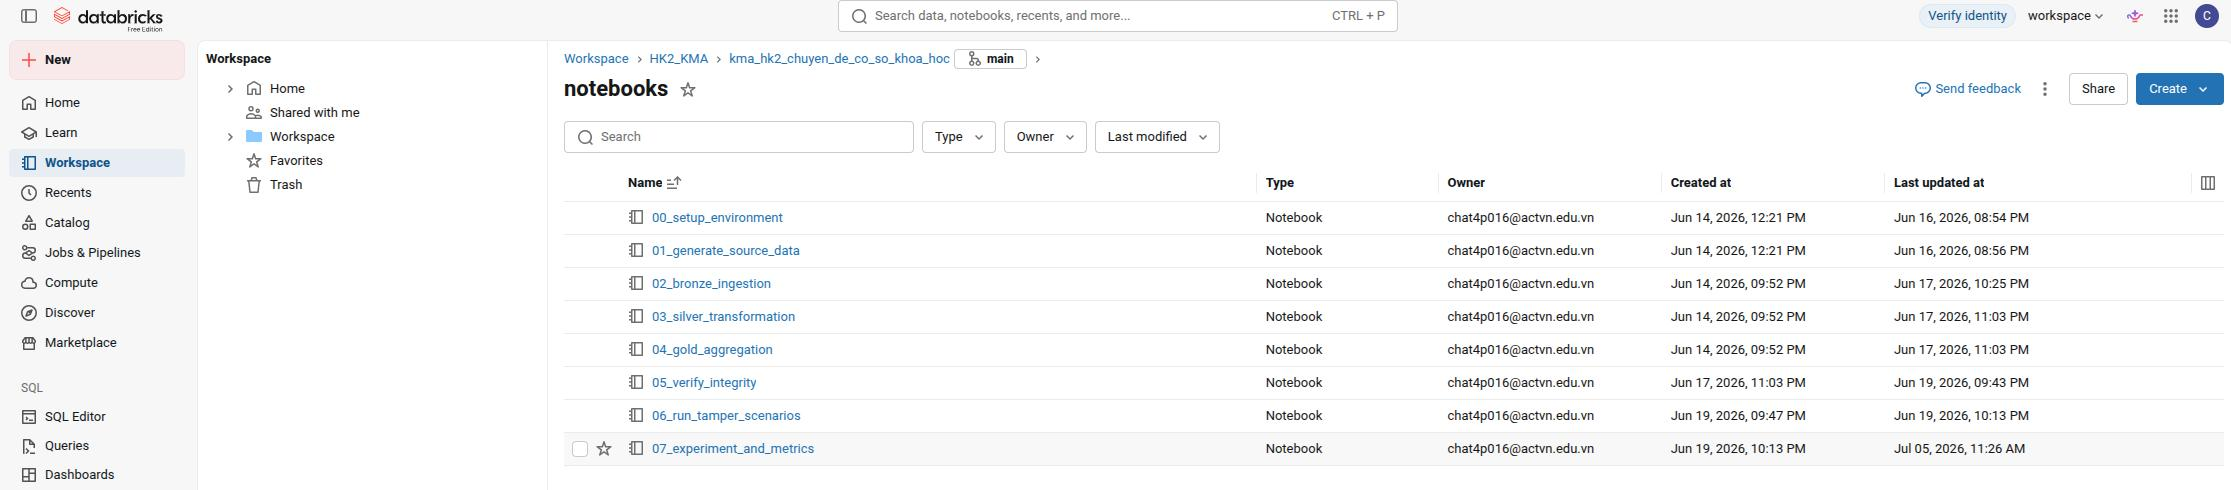
\includegraphics[width=\columnwidth]{images/screenshots/databricks_workspace_real.pdf}
\caption{Môi trường triển khai thực nghiệm trên Databricks Free Edition: các notebook \texttt{00\_setup\_environment} đến \texttt{07\_experiment\_and\_metrics} trong thư mục \texttt{notebooks}, đồng bộ từ repo Git nhánh \texttt{main}, thực thi tuần tự luồng Source--Bronze--Silver--Gold (repo: \url{https://github.com/sonnntech/kma_hk2_chuyen_de_co_so_khoa_hoc}).}
\label{fig:databricks-env}
\end{figure}

Verification engine tính toán lại bằng chứng ở từng giai đoạn và so sánh với
ledger đã lưu. Sai lệch mã băm nội dung chỉ ra khả năng data tampering. Sai
lệch số lượng bản ghi chỉ ra khả năng chèn hoặc xóa. Sai lệch block
nội dung chỉ ra ledger tampering. Sai lệch previous hash chỉ ra chain
link bị phá vỡ.

\subsection{Tamper Scenarios}\label{tamper-scenarios}

Nghiên cứu đánh giá sáu tamper scenarios và một clean scenario. Clean
scenario, ký hiệu NONE, được dùng để quan sát false positive. Các tamper
scenarios bao gồm sửa giá trị giao dịch, xóa bản ghi, chèn bản ghi giả,
sửa batch hash đã lưu, sửa transformation siêu dữ liệu và sửa previous-hash
link. Bảng~\ref{tab:scenarios} liệt kê từng scenario cùng verification
outcome kỳ vọng.

\begin{table}[!t]
\centering
\footnotesize
\caption{Tamper scenarios và outcome kỳ vọng}
\label{tab:scenarios}
\begin{tabular}{|p{3.9cm}|p{3.4cm}|}
\hline
\textbf{Scenario} & \textbf{Outcome kỳ vọng} \\
\hline
NONE & VALID \\
\hline
MODIFY\_\allowbreak TRANSACTION\_\allowbreak AMOUNT & DATA\_\allowbreak TAMPERED \\
\hline
DELETE\_\allowbreak TRANSACTION & RECORD\_\allowbreak COUNT\_\allowbreak MISMATCH \\
\hline
INSERT\_\allowbreak FAKE\_\allowbreak TRANSACTION & RECORD\_\allowbreak COUNT\_\allowbreak MISMATCH \\
\hline
MODIFY\_\allowbreak LEDGER\_\allowbreak BATCH\_\allowbreak HASH & DATA\_\allowbreak TAMPERED \\
\hline
MODIFY\_\allowbreak LEDGER\_\allowbreak TRANSFORMATION & BLOCK\_\allowbreak TAMPERED \\
\hline
MODIFY\_\allowbreak LEDGER\_\allowbreak PREVIOUS\_\allowbreak HASH & CHAIN\_\allowbreak BROKEN \\
\hline
\end{tabular}
\end{table}
\subsection{Quy trình thực
nghiệm}\label{sec:quytrinh}

Quy trình thực nghiệm được mô tả trong
Hình~\ref{fig:procedure}. Đầu tiên, môi trường và các
Delta tables được khởi tạo. Tiếp theo, dữ liệu synthetic được sinh bằng
seed cố định. Sau đó, pipeline baseline và pipeline có treatment được
thực thi. Verification engine kiểm tra clean run. Một tamper scenario
được áp dụng, rồi verification được chạy lại để đo detection và
traceability. Trạng thái baseline được reset trước khi chuyển sang
scenario tiếp theo. Cuối cùng, benchmark được chạy theo nhiều mức record
count.

\begin{figure}[t]
\centering
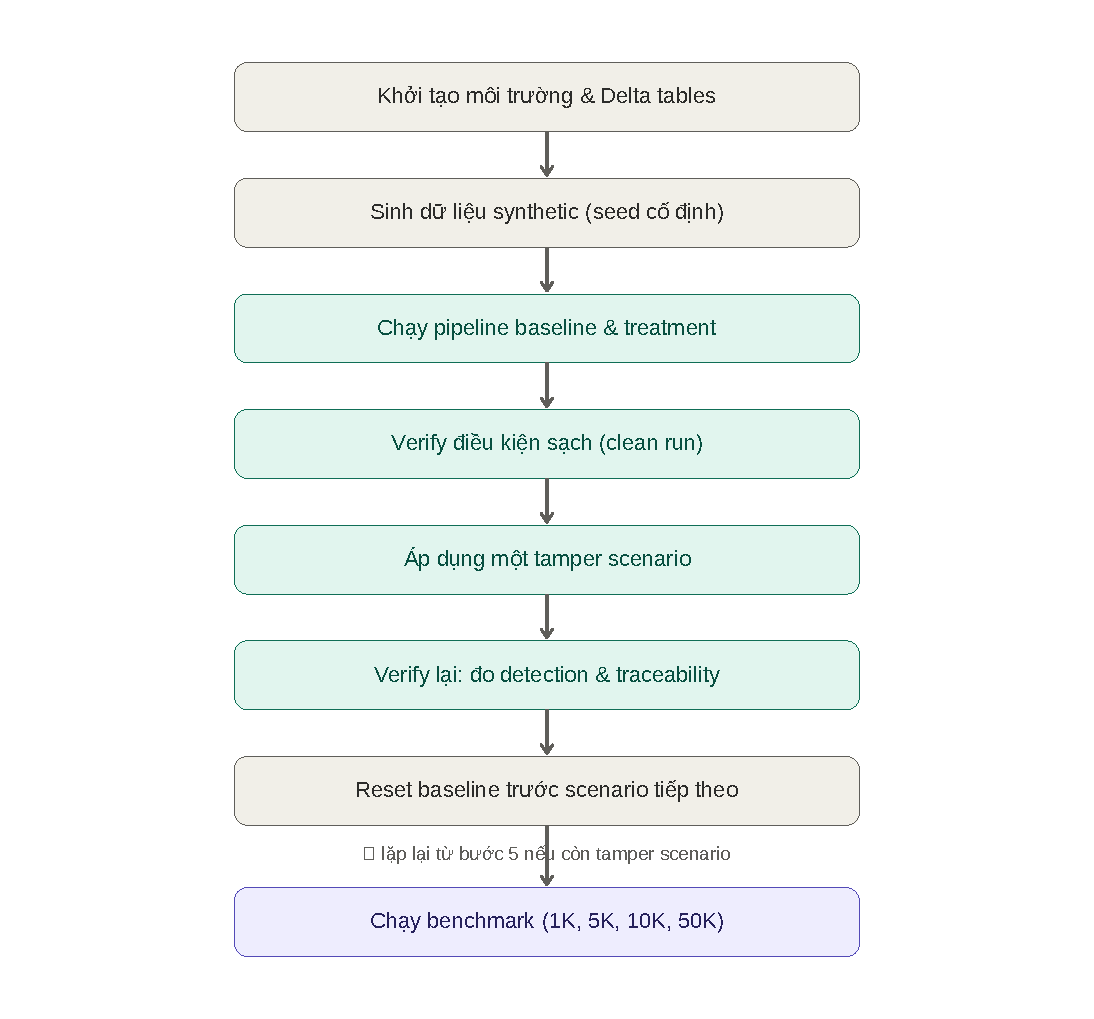
\includegraphics[width=\columnwidth]{images/quy_trinh_thuc_nghiem.pdf}
\caption{Quy trình thực nghiệm cho clean run, tamper run và benchmark run.}
\label{fig:procedure}
\end{figure}

Các lần chạy khởi động (warm-up) được đánh dấu và loại khỏi phần tổng hợp benchmark
chính. Median chi phí phát sinh được ưu tiên hơn mean vì trạng thái cloud compute
và khởi động nguội (cold start) có thể tạo giá trị ngoại lai. Benchmark sử dụng các mức số lượng bản ghi
1K, 5K, 10K và 50K.

\FloatBarrier

\section{Đánh giá thực
nghiệm}\label{sec:danhgia}

\subsection{Kết quả phát hiện
tamper}\label{sec:ketquaphathien}

Điều kiện sạch tạo ra verification outcome là VALID trong bảng điều khiển
xuất dữ liệu được dùng làm bằng chứng cho trạng thái không bị tamper. Các
tamper experiments tạo ra outcome non-VALID cho tất cả tamper scenarios
được định nghĩa trước. Bảng~\ref{tab:results} tóm tắt
các outcome quan sát được. Kết quả hỗ trợ H1 trong phạm vi bounded set
của các scenarios đã đánh giá.

\begin{table*}[t]
\centering
\caption{Kết quả verification quan sát được}
\label{tab:results}
\begin{tabular}{@{}p{3.6cm}p{4.4cm}p{1.3cm}@{}}
\toprule
\textbf{Scenario} & \textbf{Outcome quan sát} & \textbf{Loại} \\
\midrule
NONE & VALID & TN \\
MODIFY\_\allowbreak TRANSACTION\_\allowbreak AMOUNT & DATA\_\allowbreak TAMPERED & TP \\
DELETE\_\allowbreak TRANSACTION & RECORD\_\allowbreak COUNT\_\allowbreak MISMATCH & TP \\
INSERT\_\allowbreak FAKE\_\allowbreak TRANSACTION & RECORD\_\allowbreak COUNT\_\allowbreak MISMATCH & TP \\
MODIFY\_\allowbreak LEDGER\_\allowbreak BATCH\_\allowbreak HASH & DATA\_\allowbreak TAMPERED & TP \\
MODIFY\_\allowbreak LEDGER\_\allowbreak TRANSFORMATION & BLOCK\_\allowbreak TAMPERED & TP \\
MODIFY\_\allowbreak LEDGER\_\allowbreak PREVIOUS\_\allowbreak HASH & CHAIN\_\allowbreak BROKEN & TP \\
\bottomrule
\end{tabular}
\end{table*}
Detection rate được tính theo công thức:

\begin{equation}
Detection\ Rate = \frac{TP}{TP + FN} \times 100\%.
\end{equation}

Với sáu true positives và không quan sát thấy false negative trong các
tampered scenarios, detection rate đạt 100\% trong test set được định
nghĩa trước. Kết quả này không nên được hiểu là coverage phổ quát đối
với mọi attack vector. Nó chỉ có nghĩa là cơ chế đã phát hiện sáu tamper
vectors được lựa chọn trong thực nghiệm này.

\subsection{Kết quả traceability}\label{sec:traceability}

Verification engine trả về first broken block khi phát hiện mismatch.
Block này có thể được join với lineage events thông qua pipeline run
identifier. Lineage flow mẫu ghi nhận các transformation
Source-to-Bronze, Bronze-to-Silver và Silver-to-Gold, bao gồm input
số lượng bản ghi, output số lượng bản ghi, transformation context và status. Đối
với các tamper scenarios được đánh giá, first broken block và lineage
context khớp với affected giai đoạn ở mức giai đoạn tổng quát. Điều này hỗ trợ
H2, nhưng vẫn có giới hạn: một số giá trị giai đoạn trong source report được
ghi nhận ở mức approximate và cần được xác minh bằng SQL xuất dữ liệu trực
tiếp để có kết luận mạnh hơn.

\subsection{Kết quả chi phí phát sinh}\label{sec:overhead}

Security chi phí phát sinh được tính theo công thức:

\begin{equation}
\text{Chi phí phát sinh} = \frac{SecuredDuration - BaselineDuration}{BaselineDuration} \times 100\%.
\end{equation}

Các giá trị xấp xỉ từ bảng điều khiển cho thấy chi phí phát sinh tăng từ khoảng 160\% ở
mức 1K records lên khoảng 220\% ở mức 50K records.
Bảng~\ref{tab:overhead} tóm tắt xu hướng quan sát được.
Trường hợp 5K gần với 1K, cho thấy khả năng có ảnh hưởng của cloud
runtime variance. Nhìn chung, bằng chứng hỗ trợ H3 nhưng kèm caveats.

\begin{table*}[t]
\centering
\caption{Runtime chi phí phát sinh xấp xỉ theo số lượng bản ghi}
\label{tab:overhead}
\begin{tabular}{@{}p{2.7cm}p{5cm}p{5cm}@{}}
\toprule
\textbf{Số lượng bản ghi} & \textbf{Chi phí phát sinh xấp xỉ} & \textbf{Bằng chứng} \\
\midrule
1K & \(\sim\)160\% & Dashboard \\
5K & \(\sim\)155--160\% & Dashboard \\
10K & \(\sim\)180\% & Dashboard \\
50K & \(\sim\)220\% & Dashboard \\
\bottomrule
\end{tabular}
\end{table*}
Verification latency dao động xấp xỉ từ 24 giây đến 31 giây trong các
runs gần nhất, với một giá trị ngoại lai cao hơn. Quan sát này phù hợp với giả
định bán thực nghiệm rằng khởi động nguội (cold start) và cloud compute scheduling không
thể được kiểm soát hoàn toàn.

\subsection{Thảo luận}\label{sec:thaoluan}

Bằng chứng thực nghiệm cho thấy Hash-linked Ledger có thể làm cho hành
vi tamper sau xử lý trở nên quan sát được trong pipeline nhiều giai đoạn. Cơ
chế này đặc biệt hữu ích khi mục tiêu không phải là ngăn chặn trực tiếp
privileged writes, mà là phát hiện modification trái phép trong quá
trình verification về sau. Điều này phù hợp với thiết kế tamper-evident,
không phải tamper-proof.

Kết quả cũng làm rõ vai trò của thuật ngữ Blockchain. Nguyên mẫu sử dụng
hash chain lấy cảm hứng từ Blockchain, nhưng không triển khai
distributed consensus, replicated nút, mining, proof-of-work,
proof-of-stake hoặc smart contracts. Vì vậy, thuật ngữ chính xác hơn là
Hash-linked Tamper-evident Ledger. Sự phân biệt này quan trọng đối với
construct validity và giúp tránh overclaiming.

\section{Các mối đe dọa đến tính hợp
lệ}\label{sec:threats}

\subsection{Tính hợp lệ nội
tại}\label{sec:sec:validitynoitai}

Mối đe dọa chính đến tính hợp lệ nội tại là trạng thái compute không
được kiểm soát hoàn toàn. Thực nghiệm chạy trong môi trường Databricks
do cloud quản lý, trong đó cluster khởi động, trạng thái cache, cơ chế
lập lịch và phân bổ tài nguyên không cố định. Các yếu tố này có thể ảnh
hưởng đến overhead thời gian chạy độc lập với treatment. Để giảm rủi ro
này, các lần chạy khởi động (warm-up) được loại khỏi phân tích chính và
median được ưu tiên hơn mean.

Một mối đe dọa khác là hiệu ứng lịch sử. Nếu các bảng không được reset
đúng giữa các kịch bản tamper, dữ liệu cũ hoặc bản ghi ledger cũ có thể
tạo dương tính giả hoặc âm tính giả. Vì vậy, quy trình bao gồm bước
\texttt{RESET\_BASELINE} bắt buộc trước khi chuyển sang kịch bản tiếp theo.

\subsection{Tính hợp lệ ngoại
tại}\label{sec:validitingoaitai}

Thực nghiệm sử dụng một workspace Databricks và dữ liệu giao dịch tổng
hợp. Kết quả có thể không khái quát trực tiếp sang AWS Glue, Spark tại
chỗ, dbt, Snowflake hoặc môi trường lakehouse production. Dữ liệu tổng
hợp cũng thiếu các đặc điểm như phân phối lệch, trôi cấu trúc dữ liệu,
giá trị thiếu và độ phức tạp vận hành của dữ liệu thực tế. Các nghiên
cứu lặp lại trong tương lai nên triển khai trên nhiều môi trường và sử
dụng dữ liệu giống môi trường vận hành thực tế đã ẩn danh.

\subsection{Tính hợp lệ khái
niệm}\label{sec:validitykhainiem}

Hệ thống không nên được diễn giải là Blockchain đầy đủ. Khái niệm được
đánh giá trong nghiên cứu là Hash-linked Tamper-evident Ledger. Cơ chế
này cung cấp bằng chứng toàn vẹn thông qua các giá trị hash và liên kết
\texttt{previous\_hash}, nhưng không cung cấp đồng thuận phân tán hay
tính bất biến của public chain. Một mối đe dọa khái niệm khác là chỉ số
tỷ lệ phát hiện. Tỷ lệ phát hiện 100\% chỉ áp dụng cho sáu kịch bản
tamper được lựa chọn trong thực nghiệm.

\subsection{Tính hợp lệ kết
luận}\label{sec:validityketluan}

Số lượng kịch bản tamper, các mức số lượng bản ghi và số lần lặp lại đo
hiệu năng còn hạn chế. Điều này làm cho kết quả hữu ích như bằng chứng
bán thực nghiệm, nhưng chưa đủ cho kết luận thống kê mạnh. Các giá trị
overhead mang tính xấp xỉ vì được đọc từ dashboard quan sát thay vì xuất
trực tiếp từ dữ liệu benchmark thô. Cần ít nhất khoảng 30 lần chạy lặp
lại cho mỗi mức số lượng bản ghi để tính khoảng tin cậy, biểu đồ phân
phối và phân tích cỡ hiệu ứng mạnh hơn.

\section{Kết luận và hướng phát
triển}\label{sec:extra0}

Bài báo đã trình bày một đánh giá bán thực nghiệm đối với cơ chế
Hash-linked Tamper-evident Ledger nhằm kiểm chứng tính toàn vẹn dữ liệu
trong hệ thống Data Pipeline. Cơ chế này ghi nhận bằng chứng integrity ở
từng giai đoạn và liên kết các ledger blocks thông qua previous hash.
Verification engine tính toán lại số lượng bản ghi, mã băm cấu trúc dữ liệu (schema hash), batch hash,
block hash và liên kết chuỗi để phát hiện modification sau xử lý.

Các quan sát thực nghiệm hỗ trợ các giả thuyết chính trong phạm vi
bounded scope. Tất cả tamper scenarios được định nghĩa trước đều được
phát hiện, điều kiện sạch vẫn VALID trong bảng điều khiển xuất dữ liệu quan sát
được, và lineage context hỗ trợ xác định affected giai đoạn. Runtime
chi phí phát sinh tăng khi số lượng bản ghi tăng, nhưng kết quả chi phí phát sinh vẫn là
approximate và chịu ảnh hưởng bởi cloud compute variability.

Nghiên cứu nên được hiểu là bằng chứng cho một cơ chế tamper-evident
nhẹ, không phải bằng chứng về bảo mật Blockchain đầy đủ. Nguyên mẫu
không bao gồm decentralized consensus, nhiều independent nút, smart
contracts hoặc external neo tin cậy. Vì vậy, security boundary của
cơ chế hiện tại bị giới hạn trong controlled không gian làm việc setting.

Trong tương lai, nghiên cứu cần được lặp lại trên nhiều data platforms,
mở rộng tập tamper vectors thông qua kiểm thử đối kháng, tăng số lần
số lần lặp lại đo hiệu năng, xuất dữ liệu raw benchmark values, externalize ledger
sang một ranh giới tin cậy độc lập và bổ sung chữ ký số nhằm tăng
cường bằng chứng chống lại privileged người có quyền truy cập nội bộ modification.


\appendices
\section{Phụ lục tái lập kết quả}\label{sec:reproducibility}

Phụ lục này cung cấp đủ thông tin để tái lập lại thực nghiệm trong
khoảng 15 phút trên một workspace Databricks mới, theo đúng tinh thần
minh bạch và trung thực khoa học: các cấu hình chưa ghi nhận được liệt
kê rõ là \emph{chưa có bằng chứng} thay vì suy đoán.

\subsection{Mã nguồn và môi trường}

\begin{itemize}
\item \textbf{Repository:} \url{https://github.com/sonnntech/kma_hk2_chuyen_de_co_so_khoa_hoc}
\item \textbf{Nền tảng:} Databricks Free Edition; notebook Python compute hoặc serverless compute cho \texttt{notebooks/00--07}; Databricks SQL Warehouse chỉ dùng cho dashboard.
\item \textbf{Phụ thuộc cục bộ (kiểm thử):} \texttt{requirements.txt} — \texttt{pyspark>=3.5,<4.0}, \texttt{pytest>=8,<9} (Databricks Runtime đã có sẵn PySpark/Delta Lake).
\end{itemize}

\subsection{Cấu hình môi trường thực nghiệm}

\begin{table}[h]
\centering
\caption{Cấu hình môi trường (\texttt{config/demo\_config.py})}
\label{tab:repro-env}
\begin{tabular}{@{}p{3.2cm}p{4.5cm}@{}}
\toprule
\textbf{Thành phần} & \textbf{Giá trị / Nguồn} \\
\midrule
Catalog & \texttt{workspace} \\
Schema & \texttt{blockchain\_pipeline\_demo} \\
Default record count & 10\,000 \\
Random seed & 42 \\
Source system & \texttt{SCHOOL\_DEMO} \\
Benchmark record counts & 1\,000 / 5\,000 / 10\,000 / 50\,000 \\
Runs per size & 3 (+ warm-up, loại khỏi summary) \\
CPU/RAM máy chạy Databricks & \textbf{Evidence Not Found} — Databricks Free Edition/serverless compute không công bố cấu hình cố định. \\
Databricks Runtime version & \textbf{Evidence Not Found} — cần ghi lại từ workspace khi chạy lại. \\
\bottomrule
\end{tabular}
\end{table}

\subsection{Các bước tái lập (\textasciitilde15 phút)}

\begin{enumerate}
\item \textbf{Import repo:} Databricks Workspace $\to$ Repos $\to$ Add Repo $\to$ dán URL GitHub ở trên, chọn branch \texttt{main}.
\item \textbf{Chạy sạch (clean run), tuần tự bằng Python compute:}
\begin{verbatim}
notebooks/00_setup_environment.py
notebooks/01_generate_source_data.py
notebooks/02_bronze_ingestion.py
notebooks/03_silver_transformation.py
notebooks/04_gold_aggregation.py
notebooks/05_verify_integrity.py
\end{verbatim}
Kết quả kỳ vọng: \texttt{SOURCE/BRONZE/SILVER/GOLD = VALID}.
\item \textbf{Chạy một tamper scenario:} \texttt{notebooks/06\_run\_tamper\_scenarios.py} với widget \texttt{SCENARIO = MODIFY\_TRANSACTION\_AMOUNT}, \texttt{CONFIRM\_TAMPER = YES}. Reset bằng \texttt{SCENARIO = RESET\_BASELINE} trước khi đổi scenario khác.
\item \textbf{Chạy benchmark:} \texttt{notebooks/07\_experiment\_and\_metrics.py} với \texttt{RECORD\_COUNTS=1000,5000,10000,50000}, \texttt{RUNS\_PER\_SIZE=3}, \texttt{INCLUDE\_WARMUP=YES}.
\item \textbf{Xuất số liệu chính xác (khuyến nghị):} chạy KPI~8/9 trong \texttt{sql/dashboard\_queries.sql} trên \texttt{experiment\_metrics} (lọc \texttt{is\_warmup=false}) để thay các giá trị approximate trong Bảng~\ref{tab:overhead} bằng số liệu thô.
\item \textbf{Kiểm thử đơn vị cục bộ (tuỳ chọn):} \texttt{pip install -r requirements.txt \&\& pytest tests/}.
\end{enumerate}

\subsection{Known Reproducibility Gaps}

Theo đúng yêu cầu trung thực khoa học, các giới hạn sau được công khai
thay vì che giấu hoặc làm tròn số liệu:

\begin{table}[h]
\centering
\caption{Các khoảng trống về khả năng tái lập}
\label{tab:repro-gaps}
\begin{tabular}{@{}p{4cm}p{3.7cm}@{}}
\toprule
\textbf{Gap} & \textbf{Tác động} \\
\midrule
CPU/RAM và Databricks Runtime version chưa được ghi nhận & Giảm khả năng tái lập chính xác về hiệu năng; cần bổ sung khi chạy lại. \\
Bảng~\ref{tab:overhead} và Fig.~\ref{fig:overhead-chart} là giá trị approximate đọc từ dashboard chart, chưa export SQL trực tiếp & Cần chạy KPI~8/9 để lấy \texttt{avg\_overhead\_percent} và \texttt{median\_overhead\_percent} chính xác. \\
\texttt{RUNS\_PER\_SIZE = 3} & Chưa đủ mẫu cho box-plot/CDF đáng tin cậy; Fig.~\ref{fig:latency-chart} chỉ là minh họa min/điển hình/outlier, không phải phân phối đầy đủ. \\
first\_broken\_block trong Bảng~\ref{tab:results} ở mức giai đoạn tổng quát & Cần export JOIN \texttt{verification\_results} $\times$ \texttt{lineage\_events} để xác nhận chi tiết. \\
\bottomrule
\end{tabular}
\end{table}


\bibliographystyle{IEEEtran}
\bibliography{references}

\end{document}
